\documentclass[11pt,a4paper]{article}
\usepackage{fontspec}
\setmainfont{TeX Gyre Pagella}
\newfontfamily\headfont{Inter}[UprightFont=*-ExtraBold,BoldFont=*-ExtraBold,Extension=.otf,Path=/usr/share/fonts/opentype/inter/]
\usepackage[a4paper,margin=2.3cm]{geometry}
\usepackage{graphicx,booktabs,float,caption,array,xcolor,longtable}
\usepackage{xurl}
\usepackage[hidelinks]{hyperref}
\usepackage{titlesec}
\usepackage[round]{natbib}
\usepackage{setspace}
\setstretch{1.05}
\renewcommand{\topfraction}{0.9}
\renewcommand{\bottomfraction}{0.8}
\renewcommand{\textfraction}{0.1}
\renewcommand{\floatpagefraction}{0.75}
\setlength{\parindent}{0pt}
\setlength{\parskip}{0.55em}
\titleformat{\section}{\headfont\Large}{\thesection}{0.8em}{}
\titleformat{\subsection}{\headfont\large}{\thesubsection}{0.8em}{}
\captionsetup{font=small,labelfont=bf}
\urlstyle{same}
\hypersetup{pdftitle={The Known World},pdfauthor={Tristan Hotham}}

\begin{document}
\begin{center}
{\Large\bfseries The Known World\par}
\vspace{0.4em}
{\large How much of the Earth each tradition had written about,\\from the Bronze Age to 1960\par}
\vspace{1.2em}
{\large Tristan Hotham\par}
\vspace{0.3em}
{\small Independent researcher\\
ORCID: 0000-0003-4931-9349\\
DOI: https://doi.org/10.5281/zenodo.23897793\par}
\vspace{0.8em}
2026
\end{center}

\begin{quote}
\small
\begin{center}\textbf{Abstract}\end{center}
A popular animation shows the world lighting up as Europeans explored it. I rebuild that idea as a reproducible measurement. A gazetteer of 681 dated journey routes, with a coarse layer of 52 regions surveyed or settled for Europe, (16,038 waypoints), compiled for this study from published accounts, covers four traditions: Europe (571 journeys, from the Bronze Age Aegean onwards), the Islamic world (42), China (43) and Polynesian and Austronesian voyaging (25, dated by archaeology). Each journey lights the cells of an equal-area hexagonal grid (288,122 H3 cells) within a mode-dependent distance of its route, in the year of the nearest route point; small enclosed pockets are filled, and knowledge flagged as lost is removed. In the main run (journeys plus surveys and settlement) Europe's recorded world covers 14.9\% of the Earth's land after Ptolemy (AD 150), 20.0\% in 1492, 44.3\% in 1800 and 80.2\% in 1960 (63.9\% from journeys alone); half of the Earth's surface is lit by 1809 and half of its land by 1841. The nineteenth century adds the most land (23.0\%), and the fastest decade after 1400 is the 1870s. Large areas were recorded first by other traditions: 18.8 million km\textsuperscript{2} by China and 17.2 million km\textsuperscript{2}, mostly ocean, by Polynesian voyagers. Results are sensitive to the reveal distances (Europe's 1960 land share ranges from 58.1\% to 85.5\% across variants) and to the coverage of the gazetteer, which is a lower bound in the late period; the shape of the curve is robust.

\textbf{Keywords:} history of exploration; historical geography; travel accounts; Polynesian voyaging; Islamic geography; Chinese geography; H3 grid; open data
\end{quote}

\section{Introduction}
The animation ``World exploration from Europe's point of view'', widely shared online, starts from a black globe and lights each region as European voyages reach it. It captures something real, the growth of a written, mapped world, but it has two weaknesses. It leaves Europe's own neighbours dark long after Greek and Roman authors had described them, and it presents one tradition's record as if it were the world's knowledge. Every place on the map was, of course, known to the people who lived there, and most European travellers depended on local guides, pilots and interpreters.

This paper turns the animation into a measurement that can be checked and varied. It asks a narrow question: how much of the Earth's surface lies close to journeys whose accounts reached the readers of a given tradition, year by year? It answers it for Europe, the Islamic world, China and Polynesia, and it reports how the answer depends on the choices made. An interactive version lets readers play the timeline, switch the point of view and inspect any place or route (\url{https://maps.tristanhotham.com/known-world/}).

\section{Data}
\textbf{The gazetteer.} I compiled 681 journeys, mostly from English Wikipedia articles and the accounts they cite \citep{wiki}, in eight regional files (Greek and Phoenician; Roman and medieval; Atlantic and Indian Ocean; the Americas; the African interior; overland Asia; the Pacific and the polar regions; other points of view). Each entry gives a leader, sponsor, start and end years, a mode (sea, land, river, sledge, air, or a ``base'' starting world), an ordered route of waypoints each with a year, a one-sentence summary, sources, a route confidence and notes, including named local guides. Sea routes follow the coasts actually sailed, with waypoints at least every 300 km; land and river routes have a waypoint at each named place. 181 routes are marked low confidence because they are reconstructed or disputed. Starting worlds (``base'' entries, 25 in all) are dense clouds of points over an area already known at a date, such as the Bronze Age Aegean, the world of Herodotus or Ptolemy's \textit{Geography}; they stop each tradition starting from nothing. 13 entries carry a year in which the knowledge was lost (Vinland and Norse Greenland, the Phoenician circumnavigation of Africa, abandoned Pacific islands). Polynesian entries are settlement dates from archaeology and radiocarbon, not written accounts. Table~\ref{tab:data} summarises the composition.

\begin{table}[tbp]\centering\small\caption{The gazetteer: journeys by point of view and mode, and by source status.}\label{tab:data}\begin{tabular}{lrrrrrrr}\toprule Point of view & Journeys & Sea & Land & River & Sledge & Air & Base\\\midrule
Europe & 571 & 233 & 237 & 67 & 18 & 6 & 10\\
Islamic world & 42 & 13 & 18 & 1 & 0 & 0 & 10\\
China & 43 & 15 & 22 & 1 & 0 & 0 & 5\\
Polynesia & 25 & 25 & 0 & 0 & 0 & 0 & 0\\
\midrule\multicolumn{8}{p{14cm}}{Source status: read by compiler 405 (59.5\%); years confirmed 182 (26.7\%); years not confirmed 77 (11.3\%); unsourced 17 (2.5\%)}\\
\multicolumn{8}{p{14cm}}{Survey and settlement layer (Europe): 52 regions, 1734 to 1955, all with years not confirmed.}\\
\bottomrule\end{tabular}\end{table}

\textbf{Survey and settlement layer.} Journeys cannot capture the mapping of the world by systematic survey and settlement, which by the late nineteenth century covered most of the interiors that remain dark between routes. For Europe only, I added 52 region entries, each a set of Natural Earth first-level divisions (by ISO 3166-2 code) or countries, sometimes clipped to a box around their settled part, lit in a single year between 1734 and 1955: the year the region's systematic survey or general map was published in Europe, or its settler colonisation was general. Examples are the Mitchell map of the British colonies (1755), the US Public Land Survey by state (1800 to 1895), the Dominion Land Survey of the prairies (1890), the Russian General Land Survey (1800), the Trans-Siberian corridor (1905), the Jesuit survey of China published by d'Anville (1737), the Atlas of India (1870), the Conquest of the Desert in Argentina (1885), the colonial surveys of Australia (1830 to 1880) and the aerial survey of northern Canada (1955). These dates are mine, from general knowledge of the history of cartography; the cited pages were not reread for this layer, and all are marked as not confirmed. The layer is deliberately coarse and leaves the Amazon, the Sahara, central Africa and northern Siberia to the journeys. All results are also given for journeys alone.

\textbf{Merging and validation.} The regional files were merged and checked: latitudes in range, longitudes normalised, waypoint years within the journey's years and non-decreasing, and lone spikes in a route removed. 3 journeys appearing in two files were merged and 2 distinct journeys sharing an identifier renamed. Routes crossing the 180 degree meridian are unwrapped before densification and split at the meridian in the published GeoJSON.

\textbf{Source status.} Each journey carries one of four statuses. For part of the gazetteer an automatic check fetched the cited English Wikipedia article and searched its text for the start and end years: 26.7\% of journeys have both years confirmed. 59.5\% were taken by the compiler from the pages they cite and not rechecked. 11.3\% cite an article that lacks one or both years, or have dates partly from general knowledge; 2.5\% cite a page that could not be read or found. Figure~\ref{fig:status} maps the routes by status. The main results are repeated using only the first two groups (587 journeys).

\textbf{Geography.} Natural Earth 50m land, with the Natural Earth Antarctic ice shelves counted as land (land or permanent ice), countries and populated places \citep{naturalearth}; the H3 discrete global grid \citep{h3}.

\section{Methods}
\textbf{Grid.} The Earth is divided into the 288,122 cells of H3 resolution 4 (mean area 1,770 km\textsuperscript{2}, about 42 km across). A cell is land if its centre falls on land: 82,173 cells, 148.1 million km\textsuperscript{2}. Shares are area-weighted.

\textbf{Reveal.} Each route is densified to a point every 8 km, with years interpolated linearly between dated waypoints; base entries are left as point clouds. A cell is revealed by a journey when its centre lies within a distance that depends on the mode and on whether the cell is land or sea: for a ship 150 km of open sea and 40 km of land (a coast seen from the deck); 120 km either side of a land, river or sledge route; 150 km for a flight; 250 km around the points of a starting world. The cell's year for that journey is the year of the nearest qualifying route point. For each tradition, a cell's first year is the earliest over its journeys, and the journey responsible is recorded.

\textbf{Pocket fill.} Routes leave gaps between them. Every 10 years, any connected pocket of unknown cells smaller than 150 cells (about 266,000 km\textsuperscript{2}) is necessarily enclosed by known cells and is counted as known from the year its last rim cell was lit. Fill accounts for 8.5\% of Europe's known area in 1960.

\textbf{Loss.} A journey flagged as lost in year $L$ contributes the interval from its reveal year to $L$; a cell is known in year $t$ if $t$ lies in the union of the intervals of all journeys covering it. Cells covered only by lost journeys go dark again and light again if a later journey reaches them.

\textbf{Sensitivity.} The model was rerun without the survey layer, with all distances halved and increased by half, with no fill and with fills of 25 and 400 cells, with confirmed entries only, and with no starting worlds.

\section{Results}
\subsection{Europe's recorded world}
Figure~\ref{fig:maps} shows Europe's known world at eight dates and Figure~\ref{fig:curve} the share of land and surface over time. Europe starts from the Aegean (0.7\% of the land in 1400 BC). Greek colonisation, Herodotus, Alexander and the Roman geographers raise it to 6.7\% by AD 1, and Ptolemy's \textit{Geography} to 14.9\%: as a single starting world it is the largest step in the series, 6.3\% of the land in the decade of the 140s. The next millennium adds little; by 1400 the share is 19.5\% and by 1492 20.0\% of the land and 10.8\% of the surface.

The oceanic voyages then light the sea faster than the land. The surface share reaches 28.9\% by 1600 and passes half in 1809; the land share passes a quarter in 1542, half in 1841 and three quarters in 1936. Measured by century, the 1800s add the most land (23.0\%), followed by the 1900s (12.9\%) and the 1700s (12.8\%); the fastest decade after 1400 is the 1870s (5.9\%), when the crossings of the African interior coincided with the surveys of India and the American West. In 1960 80.2\% of the land and 66.0\% of the surface are lit. From journeys alone the corresponding figures are 39.4\% in 1800, 58.0\% in 1900 and 63.9\% in 1960, with half of the land lit by 1861; the survey and settlement layer adds 16.3\% of the world's land by 1960. Figure~\ref{fig:when} maps the period in which each place was first lit.

\begin{figure}[tbp]\centering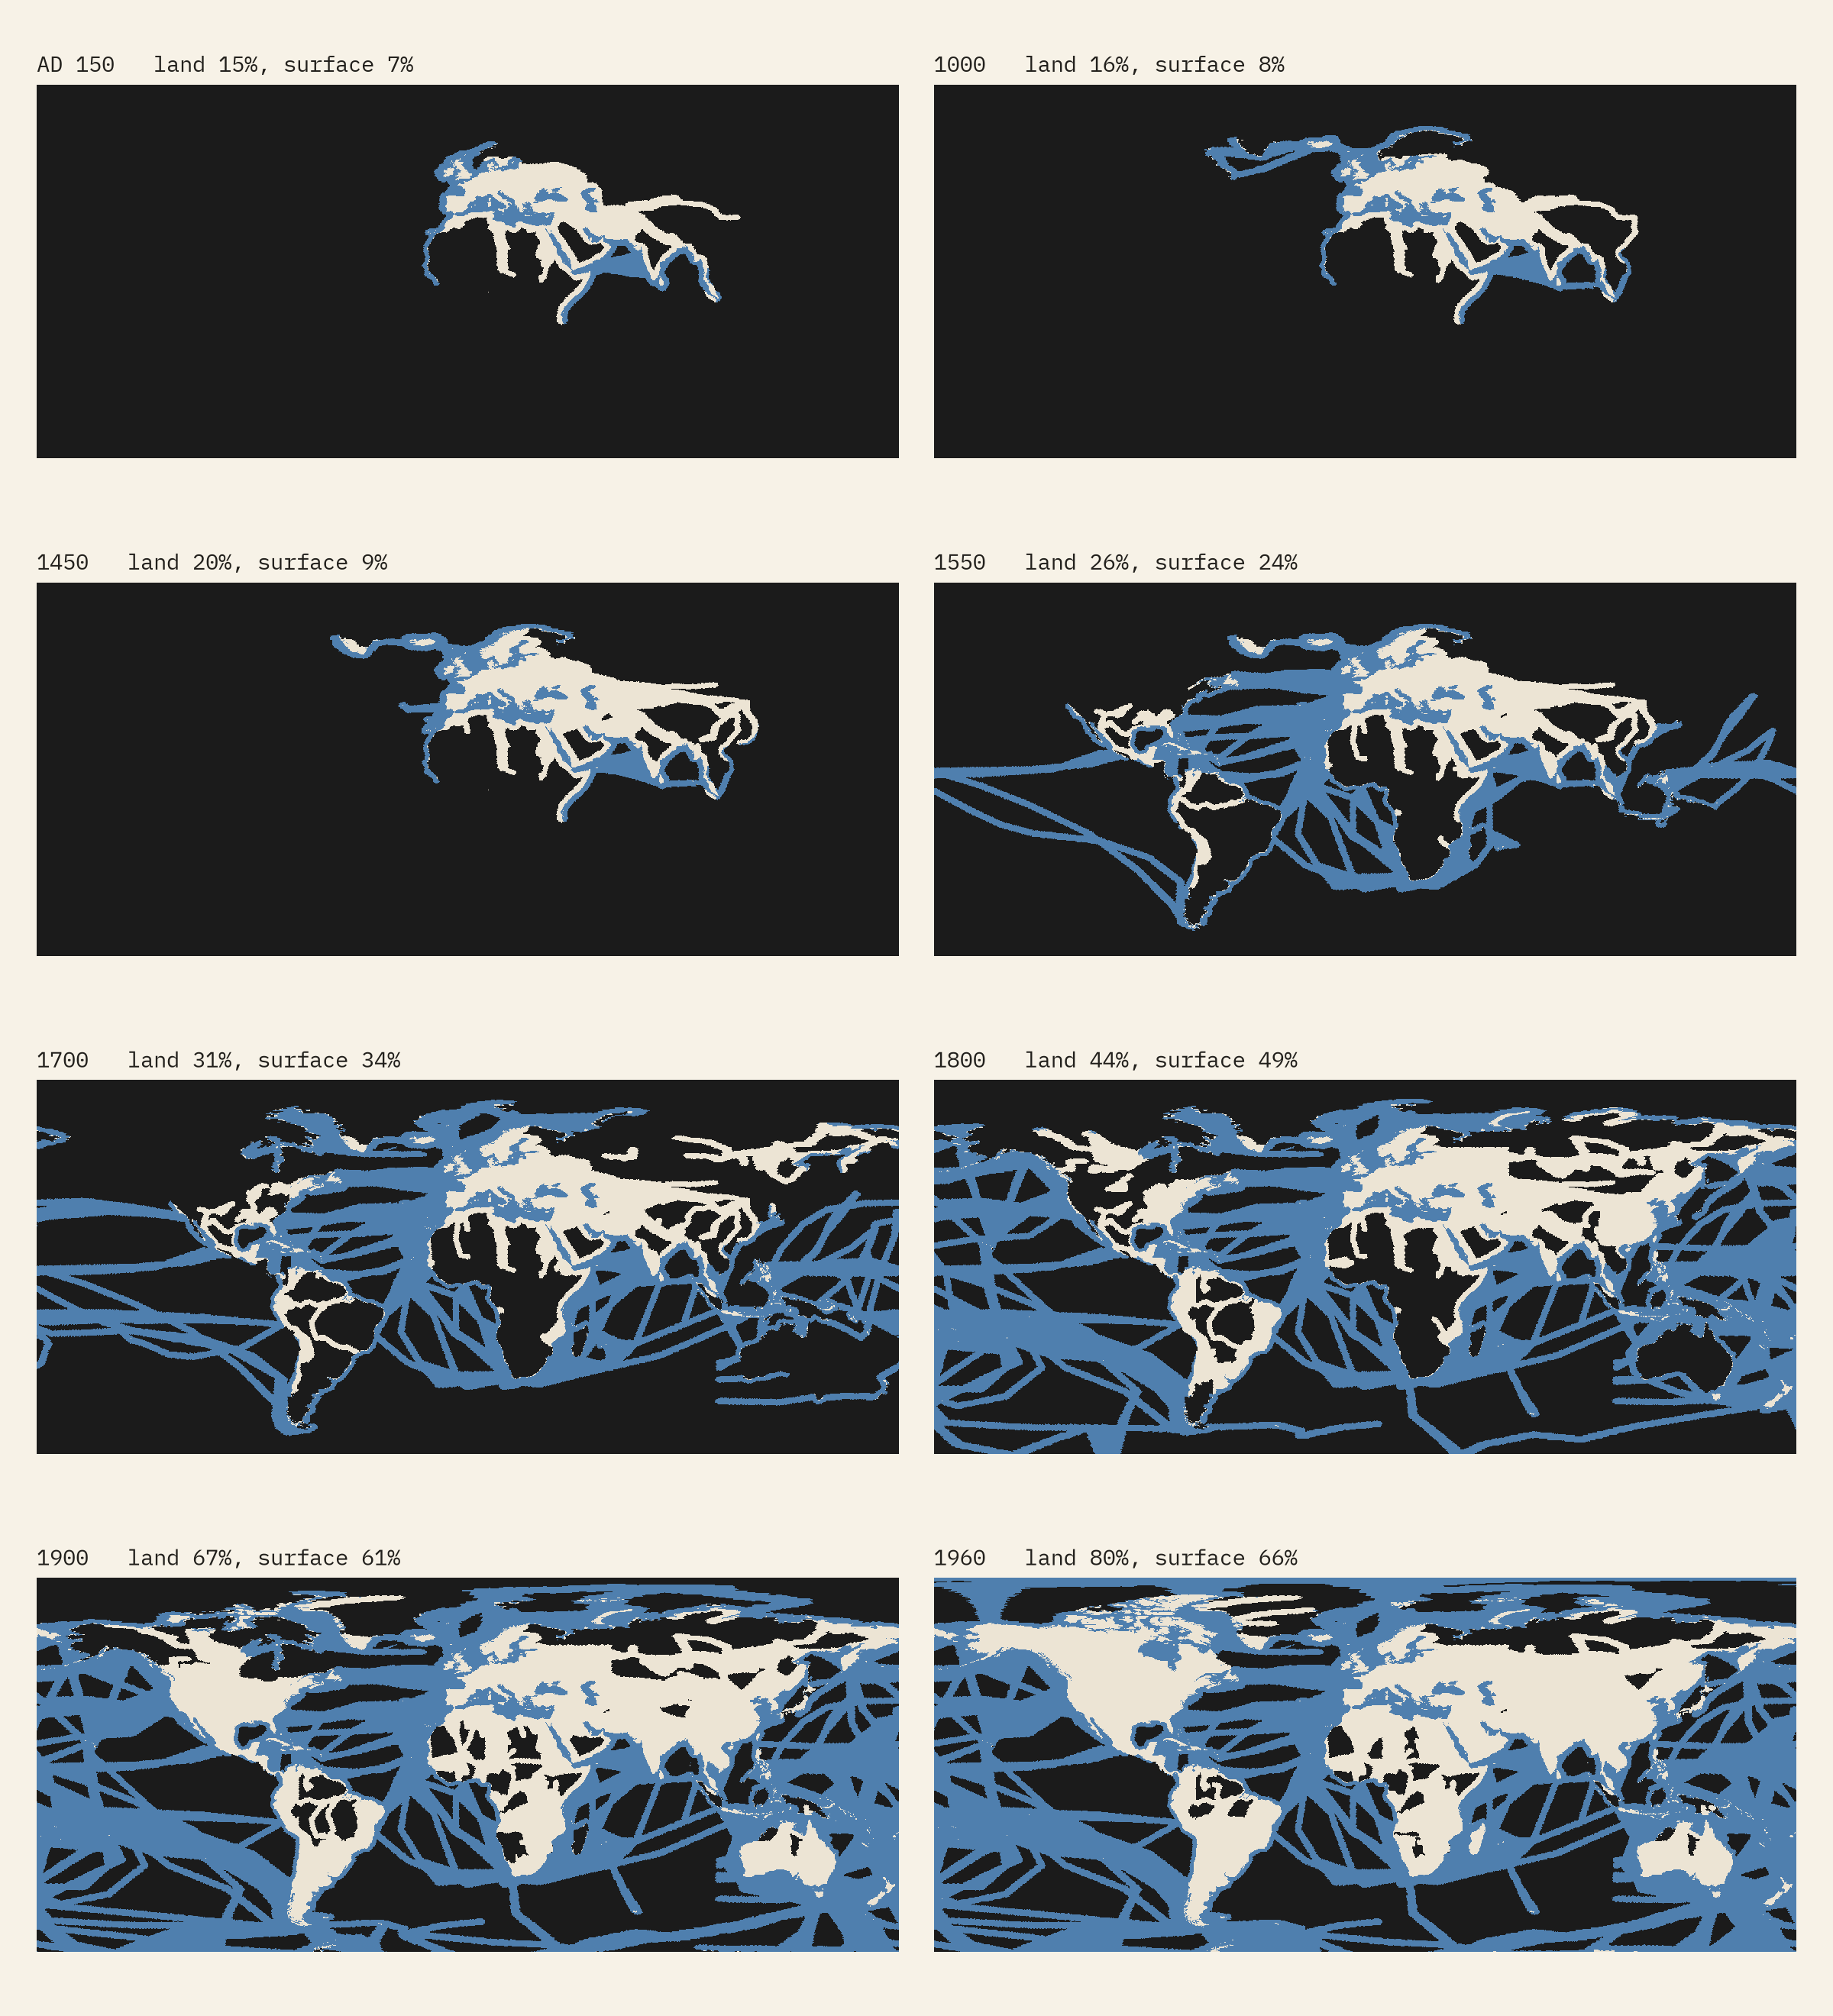
\includegraphics[width=\textwidth]{f_maps.png}
\caption{Europe's known world at eight dates: land known (cream), sea known (blue), not yet recorded for Europe (black). Titles give the share of the Earth's land and surface known.}\label{fig:maps}\end{figure}

\begin{figure}[tbp]\centering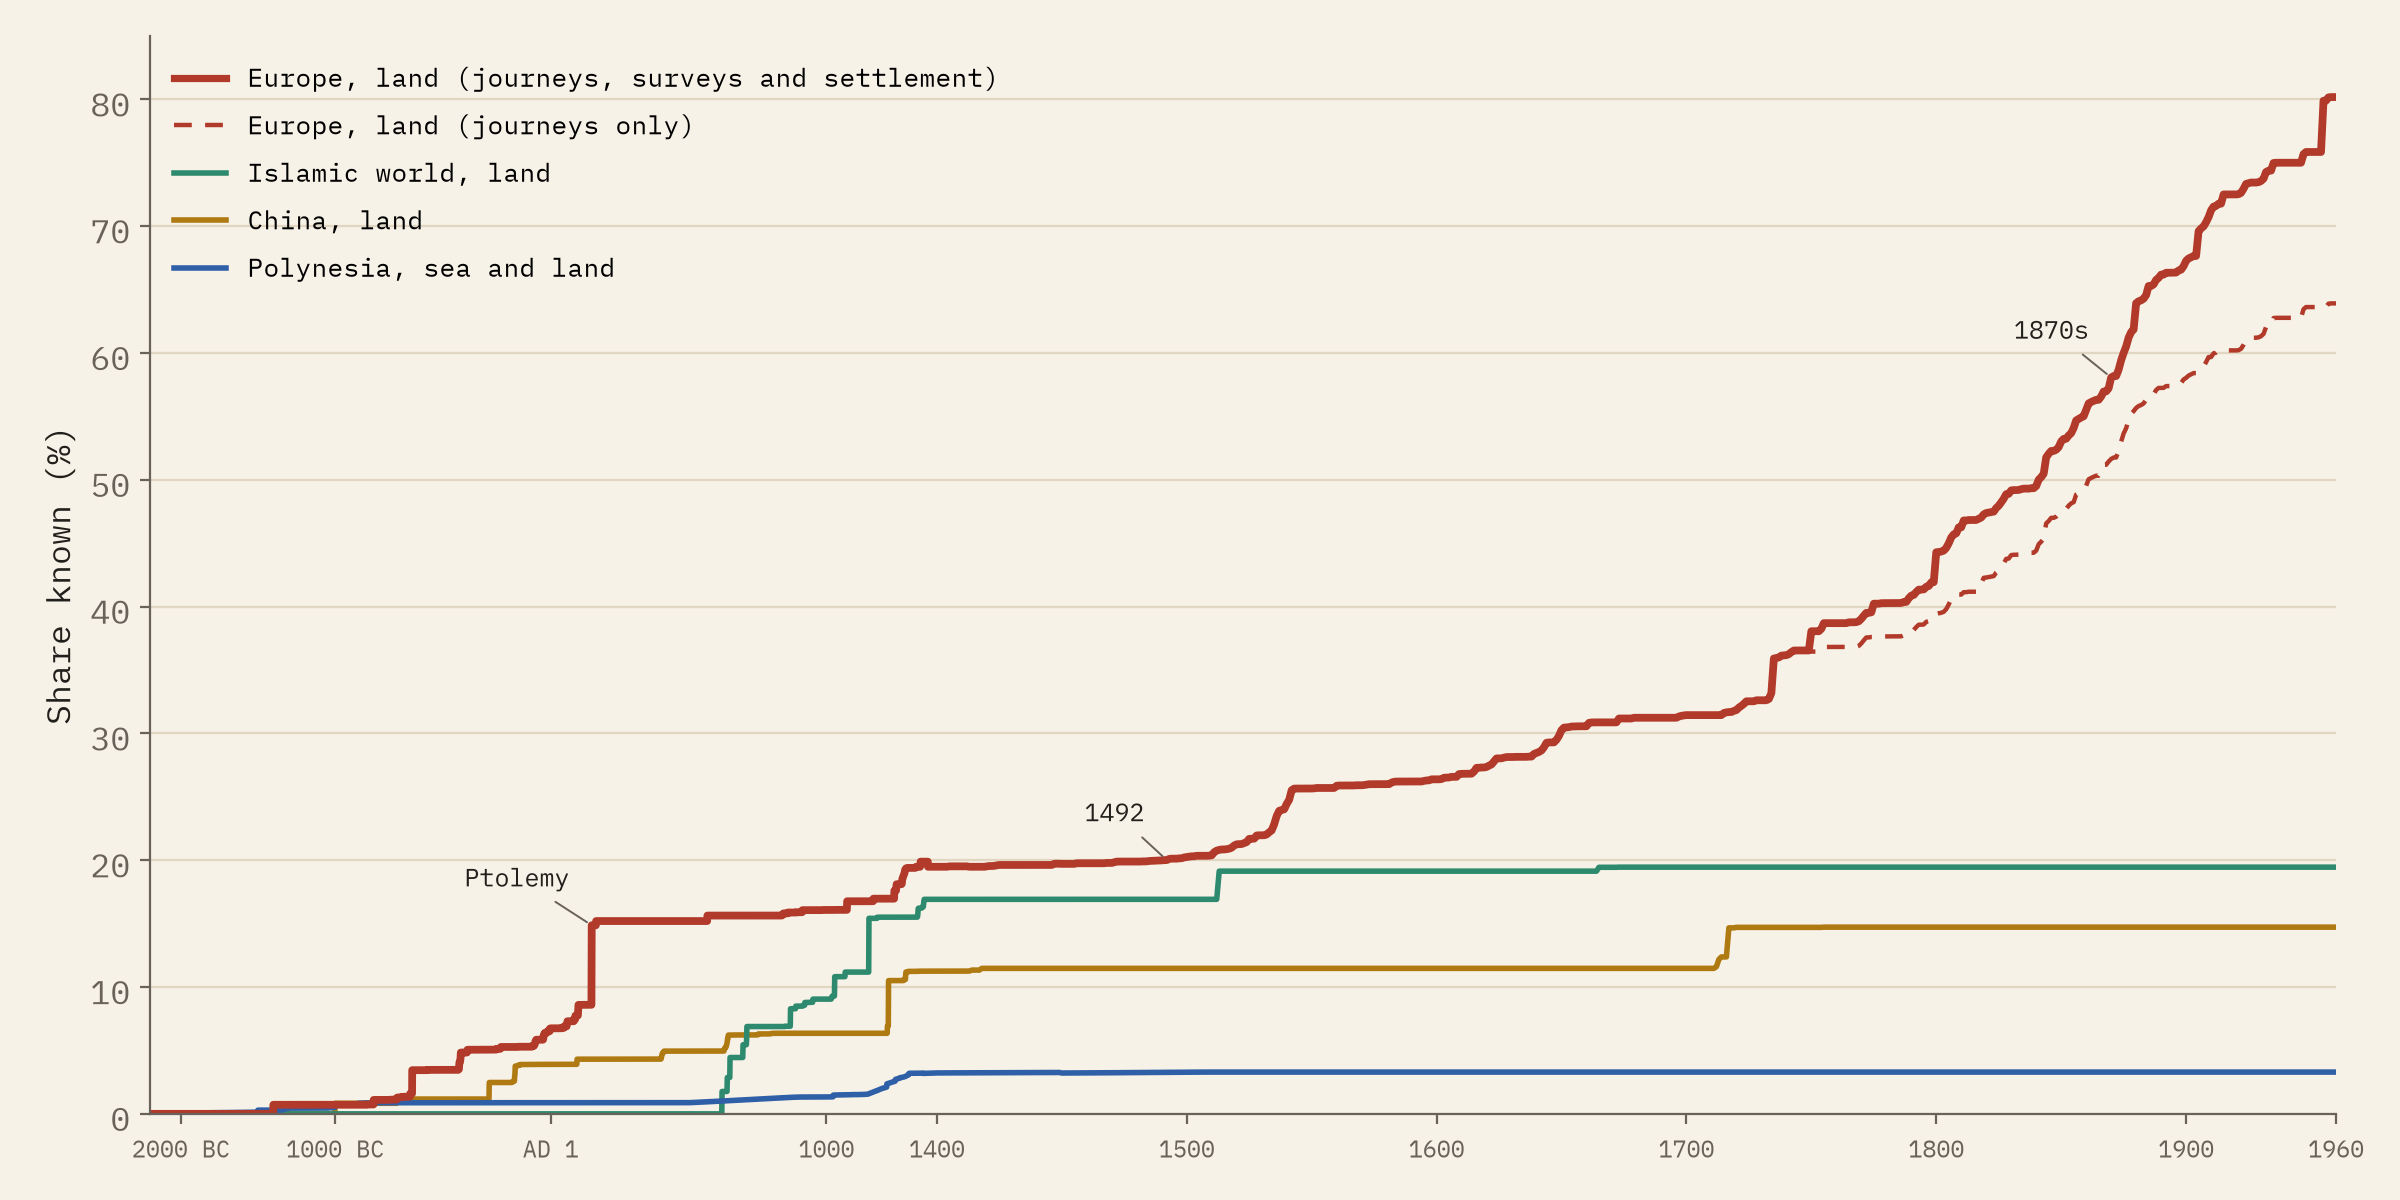
\includegraphics[width=\textwidth]{f_curve.png}
\caption{Share of the world's land known to each tradition, by year; for Polynesia, whose world was mostly ocean, the share of the whole surface. Dashed: Europe from journeys alone. The time axis is compressed before 1400.}\label{fig:curve}\end{figure}

\begin{figure}[tbp]\centering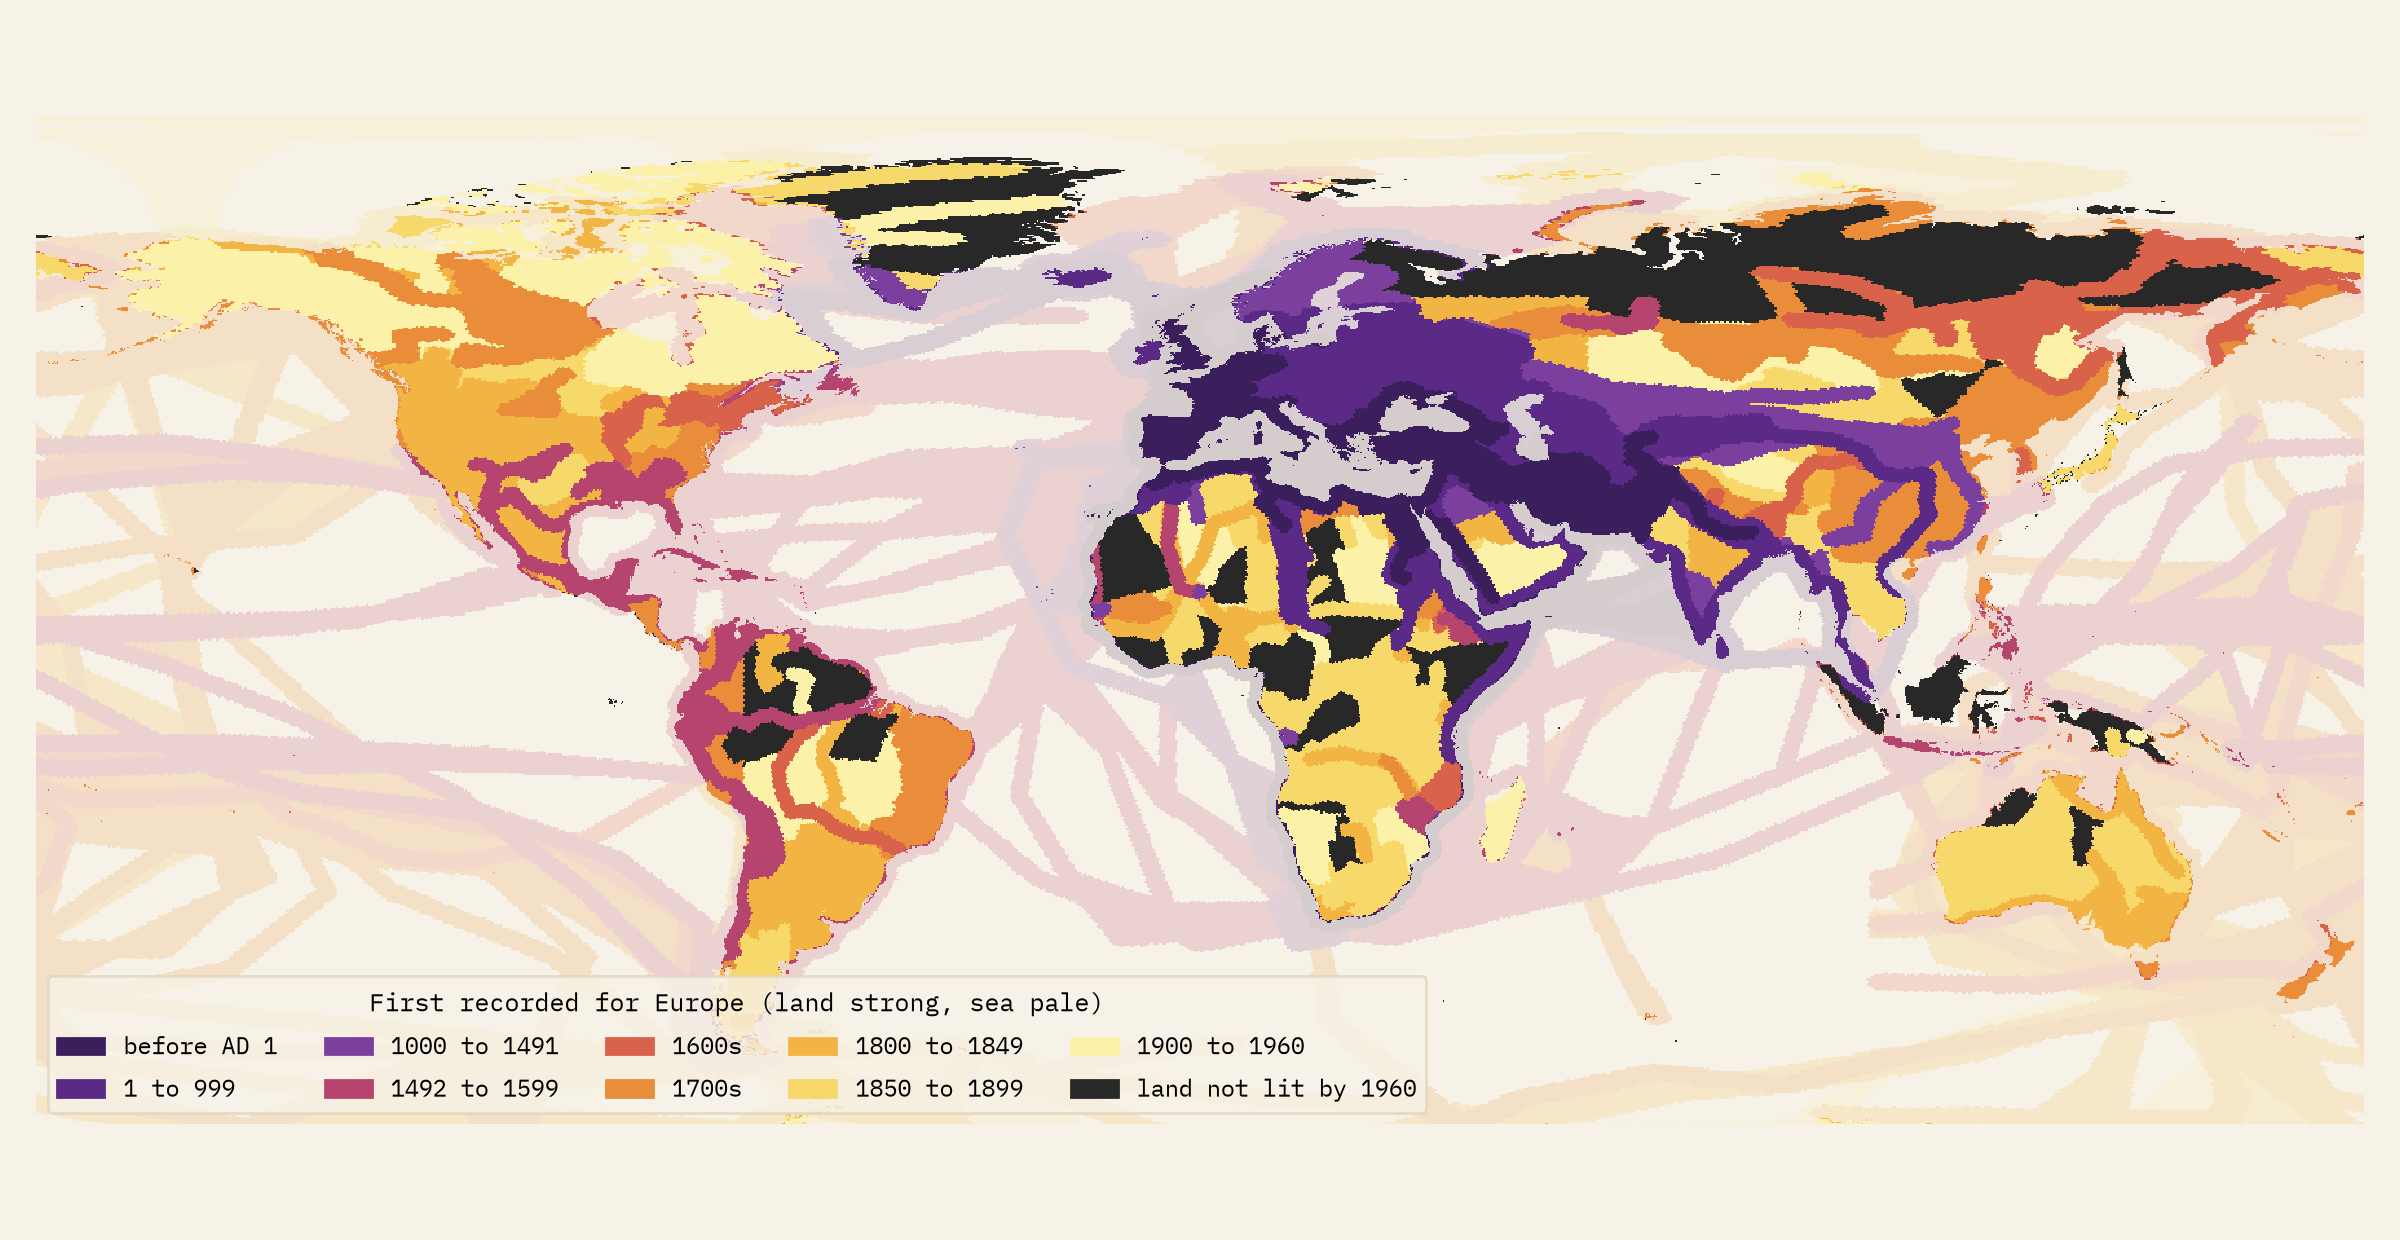
\includegraphics[width=\textwidth]{f_when.png}
\caption{When each place was first lit for Europe (land in strong colours, sea pale). Dark grey: land not lit by 1960.}\label{fig:when}\end{figure}

\subsection{The biggest journeys}
Table~\ref{tab:big} lists the journeys that first lit the largest areas for Europe, excluding starting worlds. The largest are ocean voyages, led by James Cook (1773, 8.7 million km\textsuperscript{2}) and Ferdinand Magellan; Juan Sebastian Elcano (1520, 6.9 million km\textsuperscript{2}); the ten largest together account for 17.9\% of the area known in 1960. On land the largest are John C. Fremont (1843), Agents of Maes Titianus (around AD 100) and Daniel Gottlieb Messerschmidt (1719), each over a million km\textsuperscript{2}. Because the first journey to pass a place takes all the credit, these figures reward early and wide-ranging routes rather than the depth of an account.

\begin{table}[tbp]\centering\small\caption{Journeys that first lit the largest areas for Europe (million km\textsuperscript{2}), the ten largest overall and the ten largest on land.}\label{tab:big}\begin{tabular}{lrrr}\toprule Journey & Years & New area & of it land\\\midrule
James Cook & 1773 to 1775 & 8.7 & 0.05\\
Ferdinand Magellan; Juan Sebastian Elcano & 1520 to 1522 & 6.9 & 0.03\\
James Cook & 1772 to 1773 & 6.1 & 0.00\\
Alvaro de Mendana de Neira & 1567 to 1569 & 6.1 & 0.03\\
Vasco da Gama & 1497 to 1499 & 5.9 & 0.01\\
Jean-Francois de Galaup, comte de La Perouse & 1786 to 1787 & 5.7 & 0.01\\
Alvaro de Saavedra Ceron & 1527 to 1529 & 5.6 & 0.12\\
James Cook & 1769 to 1770 & 5.4 & 0.35\\
Fabian Gottlieb von Bellingshausen; Mikhail Lazarev & 1819 to 1821 & 4.9 & 0.00\\
Garcia Jofre de Loaisa; Toribio Alonso de Salazar & 1526 & 4.9 & 0.00\\
John C. Fremont & 1843 to 1844 & 1.5 & 1.50\\
Marco Polo & 1276 to 1291 & 1.3 & 1.24\\
Agents of Maes Titianus & AD 100 to AD 102 & 1.3 & 1.25\\
Daniel Gottlieb Messerschmidt & 1719 to 1725 & 1.3 & 1.25\\
Diego de Almagro & 1535 to 1537 & 1.1 & 1.02\\
Johann Georg Gmelin and Gerhard Friedrich Muller & 1733 to 1736 & 1.1 & 1.06\\
Pyanda (Demid Pyanda) & 1620 to 1624 & 1.0 & 0.99\\
Francisco de Orellana & 1541 to 1542 & 1.0 & 0.94\\
Giovanni da Pian del Carpine (with Benedict the Pole) & 1245 to 1247 & 0.9 & 0.93\\
Antonio Raposo Tavares & 1648 to 1651 & 0.9 & 0.92\\
\bottomrule\end{tabular}\end{table}

\begin{figure}[tbp]\centering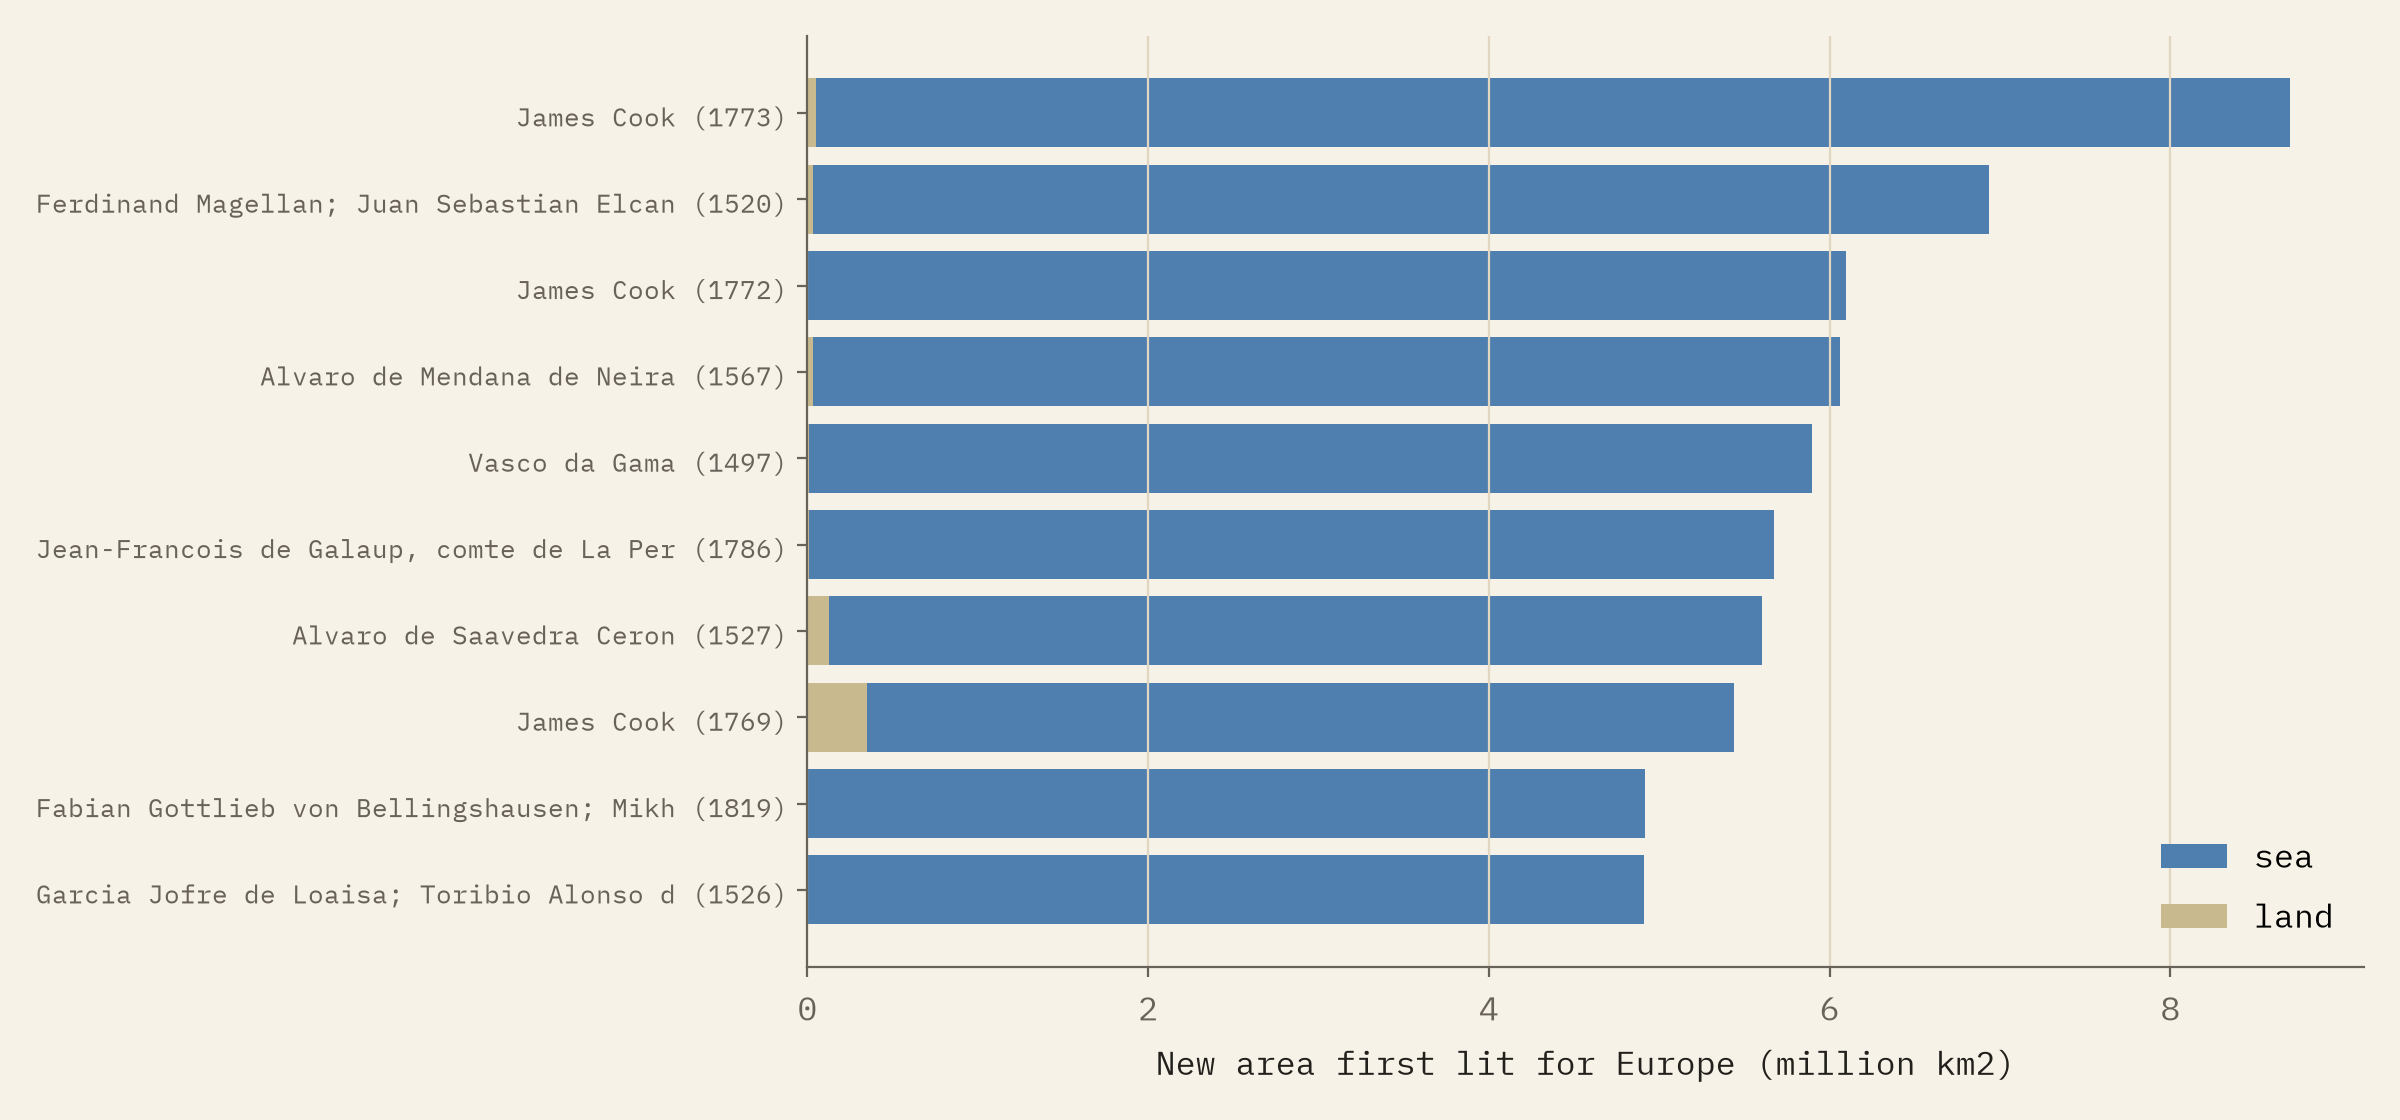
\includegraphics[width=\textwidth]{f_journeys.png}
\caption{The ten journeys that first lit the largest areas for Europe (sea and land), excluding starting worlds.}\label{fig:journeys}\end{figure}

\subsection{Other points of view}
Figure~\ref{fig:viewpoints} shows the four traditions in 1450. The Islamic world's written geography, starting from the Arabian, Syrian, Iraqi, Iranian and North African heartlands in the seventh and eighth centuries and extended by travellers and geographers to al-Andalus, the Volga, India, China and the Swahili coast, covers 16.9\% of the land in 1400. China's, from Zhang Qian's mission (138 BC) through Buddhist pilgrims to Zheng He's fleets, covers 11.5\% in 1492. Polynesian and Austronesian voyaging lights 3.2\% of the surface by 1400, almost all of it ocean (0.3\% of the land). In this gazetteer Europe leads China on land from 599 BC and is never behind the Islamic world; but in the confirmed-only run, which drops Ptolemy's \textit{Geography} among others, the Islamic world leads until 1535. Which tradition ``knew more'' before 1500 therefore rests on how a classical compilation is counted.

Table~\ref{tab:before} and Figure~\ref{fig:before} show the areas lit for another tradition before Europe. China recorded 18.8 million km\textsuperscript{2} before Europe, 55.7\% of all it recorded, a median 616 years earlier; the Islamic world 12.3 million km\textsuperscript{2} (median lead 462 years); Polynesia 17.2 million km\textsuperscript{2}, all of what it recorded, a median 555 years earlier. Hawaii was settled around 1219 and first seen by Europeans in 1778, Rapa Nui around 1250 against 1722, Aotearoa New Zealand around 1281 against 1642. Some Islamic-world leads are artefacts of the model: Piri Reis's world map of 1513, a starting-world entry compiled from European charts, lights the Brazilian coast with the 250 km base radius, more widely than the ship tracks that preceded it.

\begin{table}[tbp]\centering\small\caption{Area lit for another tradition before Europe (million km\textsuperscript{2}), median lead in years, and the countries with most such land.}\label{tab:before}\begin{tabular}{lrrrrp{6cm}}\toprule Tradition & Total & Land & Sea & Lead & Countries (land, thousand km\textsuperscript{2})\\\midrule
Islamic world & 12.3 & 8.9 & 3.4 & 462 & Brazil 1,234, Saudi Arabia 925, India 831, Mali 828\\
China & 18.8 & 13.0 & 5.8 & 616 & China 7,069, Russia 1,188, Mongolia 1,055, Indonesia 625\\
Polynesia & 17.2 & 0.4 & 16.7 & 555 & New Zealand 268, Papua New Guinea 32, Indonesia 28, Fiji 22\\
\bottomrule\end{tabular}\end{table}

\begin{figure}[tbp]\centering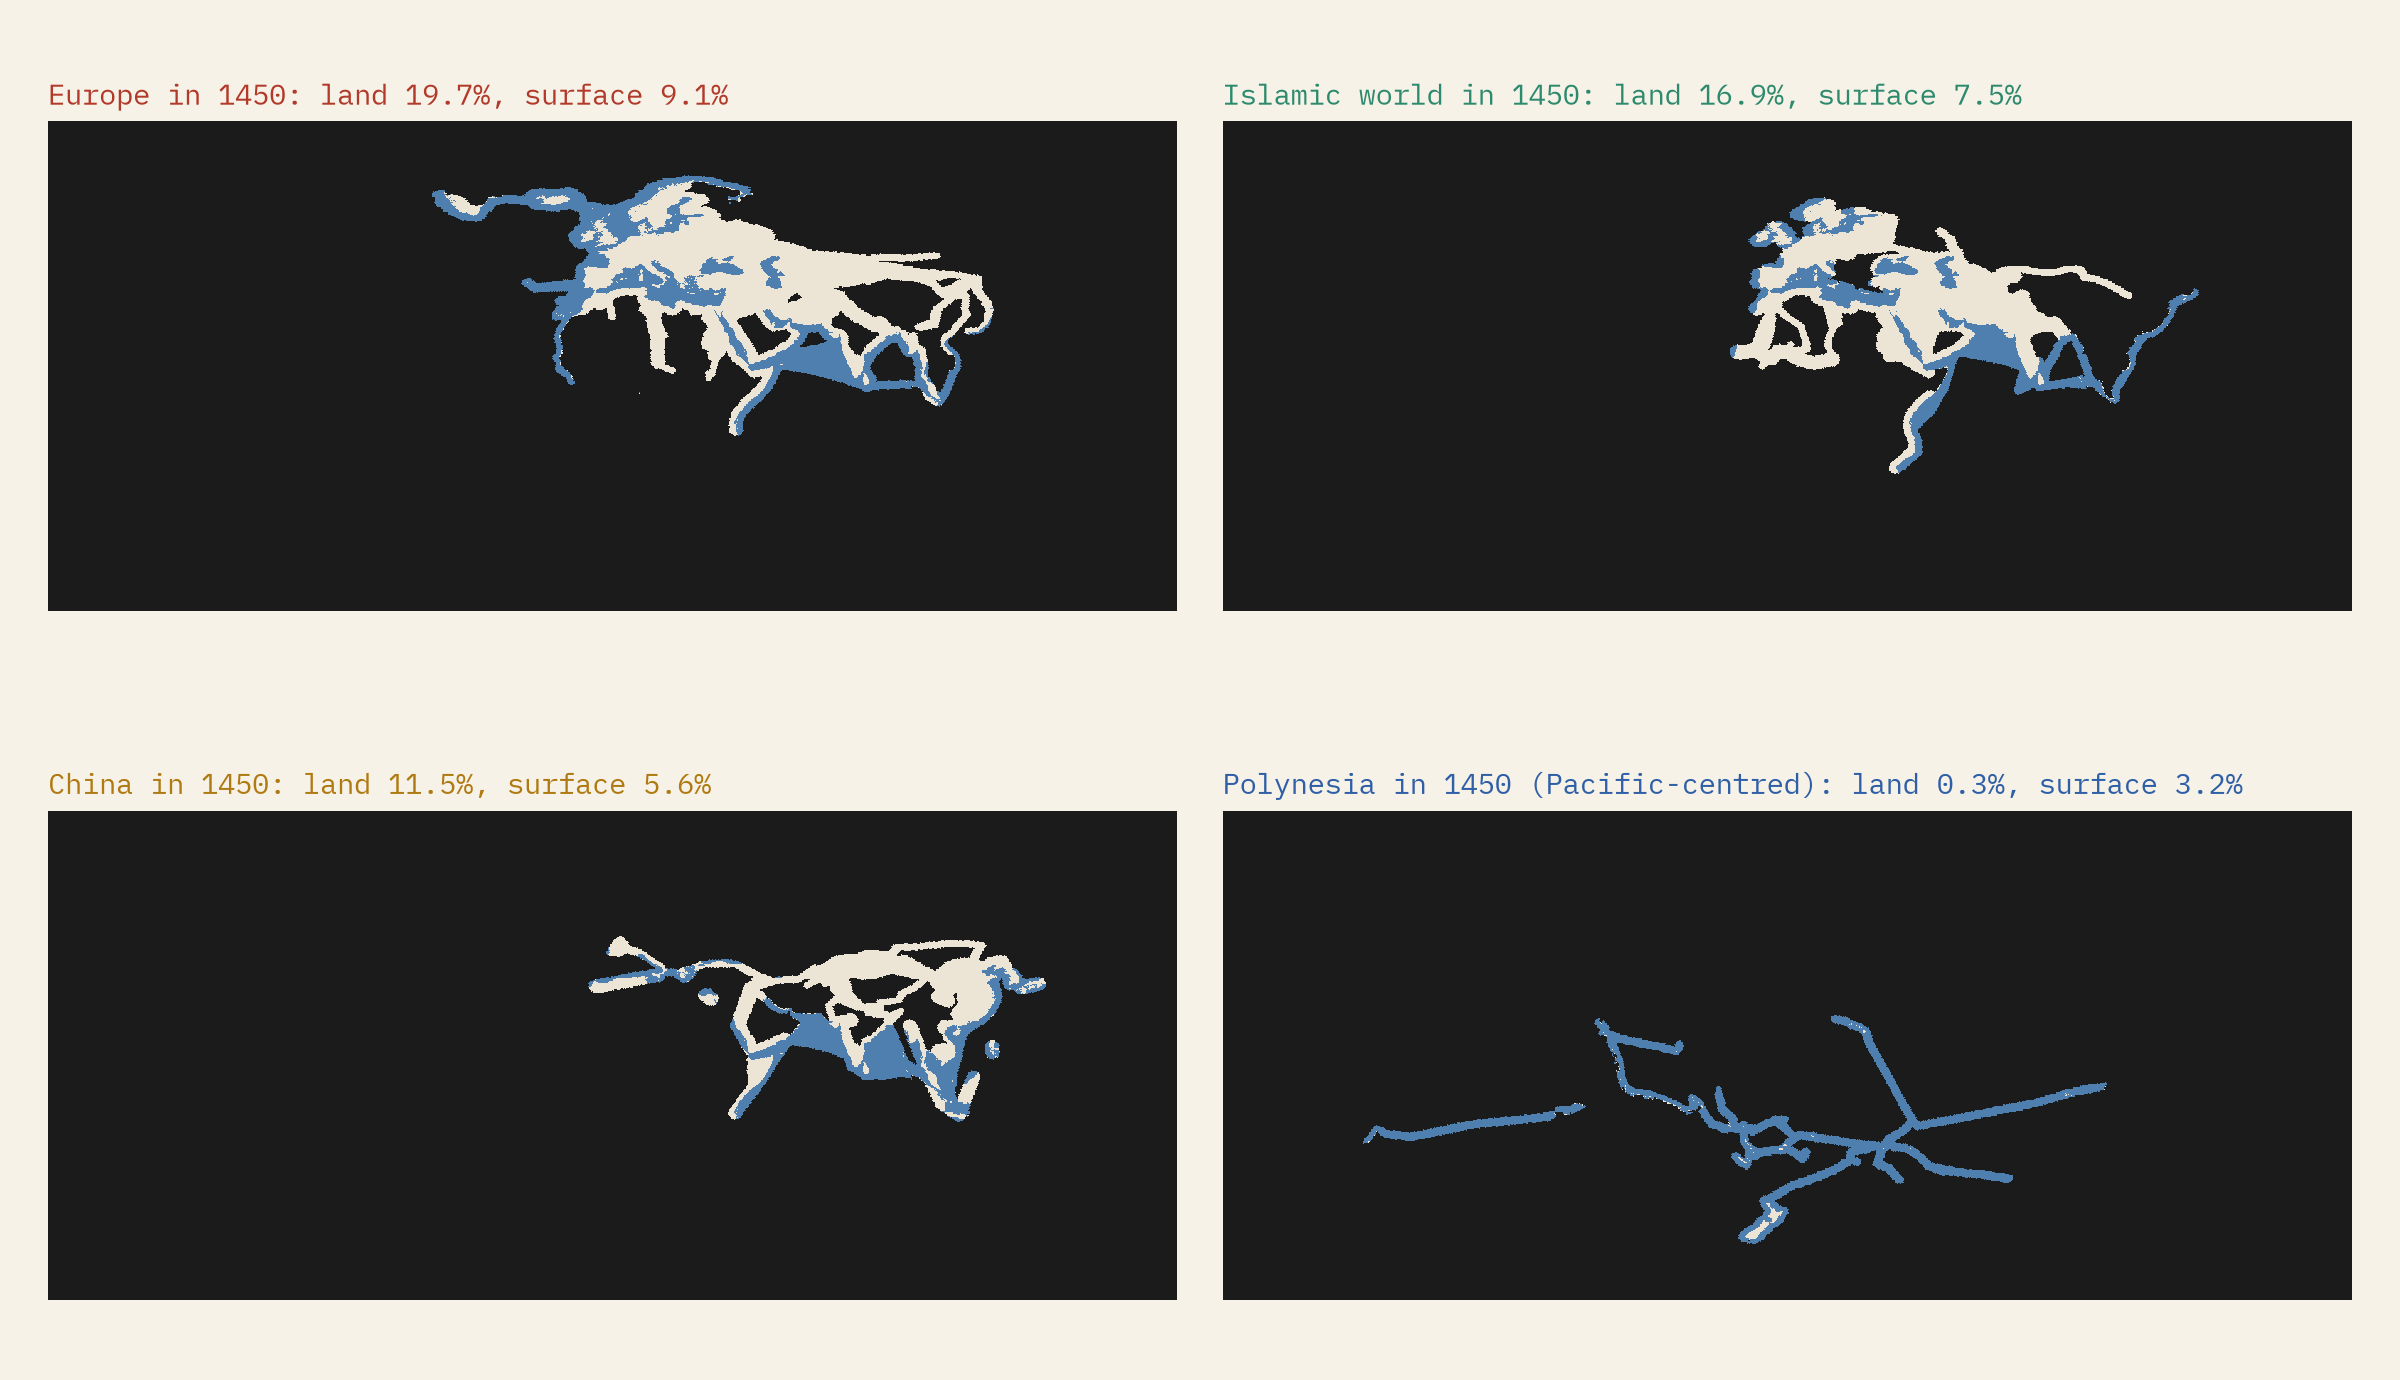
\includegraphics[width=\textwidth]{f_viewpoints.png}
\caption{The four traditions in 1450 (the Polynesian panel is centred on the Pacific).}\label{fig:viewpoints}\end{figure}

\begin{figure}[tbp]\centering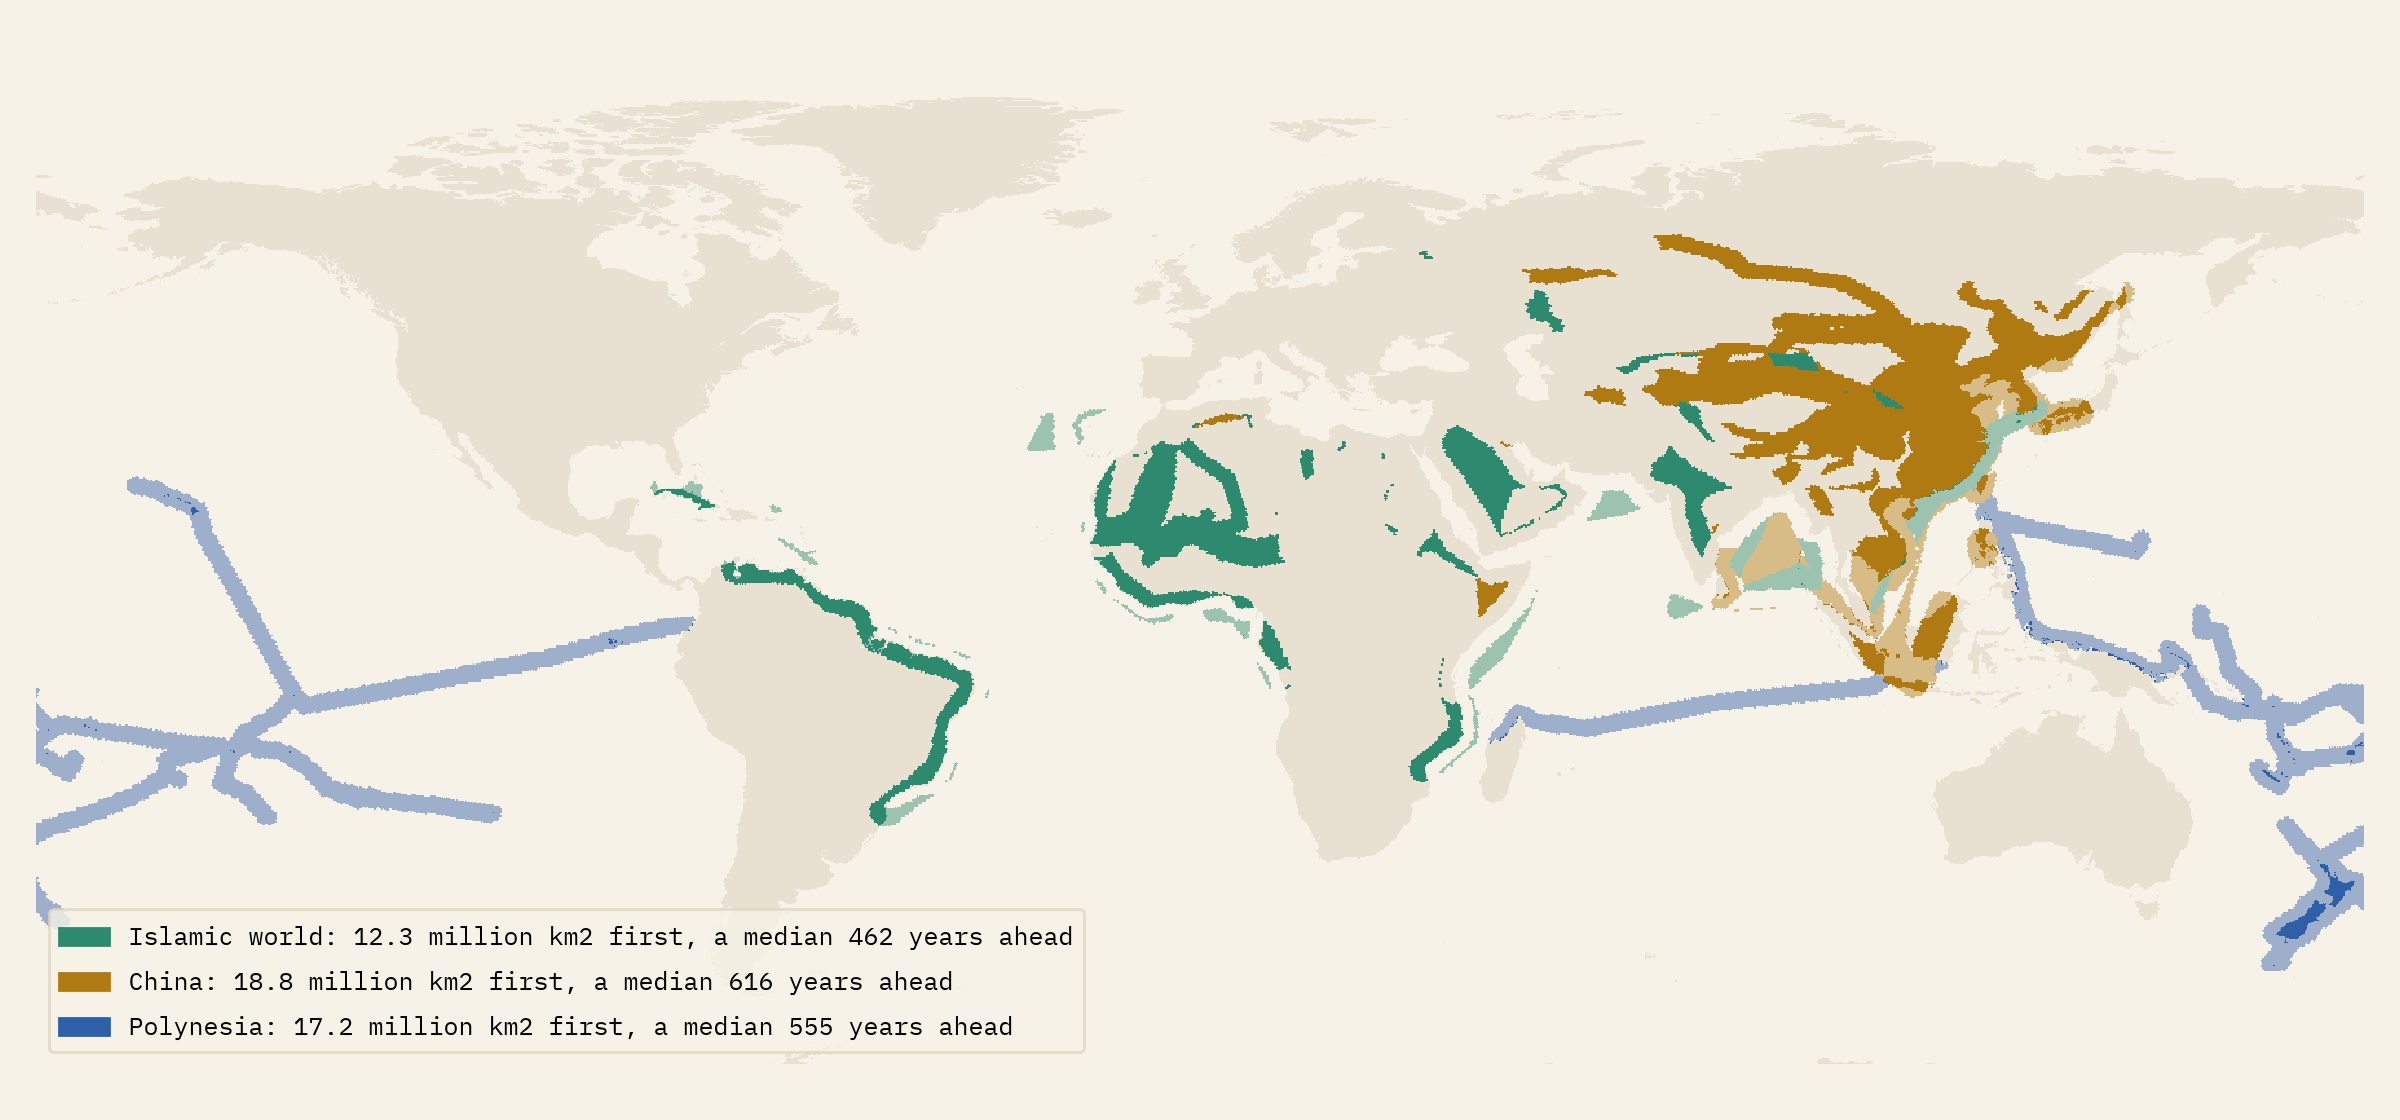
\includegraphics[width=\textwidth]{f_before.png}
\caption{Areas lit for another tradition before they were lit for Europe (or never lit for Europe by 1960). Land strong, sea pale.}\label{fig:before}\end{figure}

\subsection{The last blanks}
By the year in which half of a country's land was lit for Europe (countries over 150,000 km\textsuperscript{2}), the last are Papua New Guinea (1933), Canada (1921, its north by aerial survey), Namibia (1910) and Madagascar (1905). 19.7 million km\textsuperscript{2} of land was first lit after 1900, led by Canada, Antarctica, Brazil and the United States (Alaska). In 1960 29.4 million km\textsuperscript{2} of land remains dark (53.5 million from journeys alone), 10.4 million of it in Antarctica. Much of the rest is a gap in the data rather than in knowledge: the least-lit countries in 1960 include Cameroon, Mauritania, Indonesia and Central African Rep., which neither a journey in the gazetteer nor the coarse survey layer reaches.

\subsection{Sensitivity}
Table~\ref{tab:sens} and Figure~\ref{fig:sens} compare the variants. Distances matter most: halving them lowers Europe's 1960 land share to 72.0\%, and increasing them by half raises it to 85.5\%. The fill matters less (76.3\% without it, 85.5\% with pockets up to 400 cells). Without the survey layer the 1960 figure is 63.9\%. Keeping only confirmed entries (587 journeys, which also drops the survey layer) gives 58.1\% in 1960 and moves the half-land year from 1841 to 1877; dropping starting worlds lowers the ancient shares sharply (AD 150: 7.7\% against 14.9\%) and moves the fastest decade to the 1870s. In every variant the curve has the same shape: a slow millennium, a rise after 1492 led by the sea, and the largest land gains in the nineteenth century.

\begin{table}[tbp]\centering\small\caption{Sensitivity: Europe's share of the land known (\%) by year, the years a quarter and half of the land were lit, and the year Europe overtook China and the Islamic world on land (none: never behind).}\label{tab:sens}\begin{tabular}{lrrrrrrrrr}\toprule Variant & 150 & 1492 & 1800 & 1900 & 1960 & 25\% & 50\% & China & Islamic\\\midrule
Main run (with surveys) & 14.9 & 20.0 & 44.3 & 67.3 & 80.2 & 1542 & 1841 & 599 BC & none\\
Journeys only & 14.9 & 20.0 & 39.4 & 58.0 & 63.9 & 1542 & 1861 & 599 BC & none\\
Distances halved & 9.4 & 13.9 & 34.9 & 58.6 & 72.0 & 1735 & 1878 & 514 BC & none\\
Distances x 1.5 & 18.4 & 23.9 & 52.3 & 74.0 & 85.5 & 1512 & 1796 & 750 BC & none\\
No pocket fill & 14.4 & 19.3 & 42.2 & 64.0 & 76.3 & 1603 & 1850 & 599 BC & none\\
Fill up to 25 cells & 14.5 & 19.5 & 42.8 & 64.9 & 77.2 & 1561 & 1845 & 599 BC & none\\
Fill up to 400 cells & 14.9 & 20.0 & 46.4 & 72.1 & 85.5 & 1541 & 1825 & 599 BC & none\\
Confirmed entries only & 8.4 & 16.0 & 35.6 & 52.8 & 58.1 & 1644 & 1877 & 500 BC & 1535\\
No starting worlds & 7.7 & 14.8 & 39.3 & 64.5 & 77.7 & 1649 & 1857 & none & none\\
\bottomrule\end{tabular}\end{table}

\begin{figure}[tbp]\centering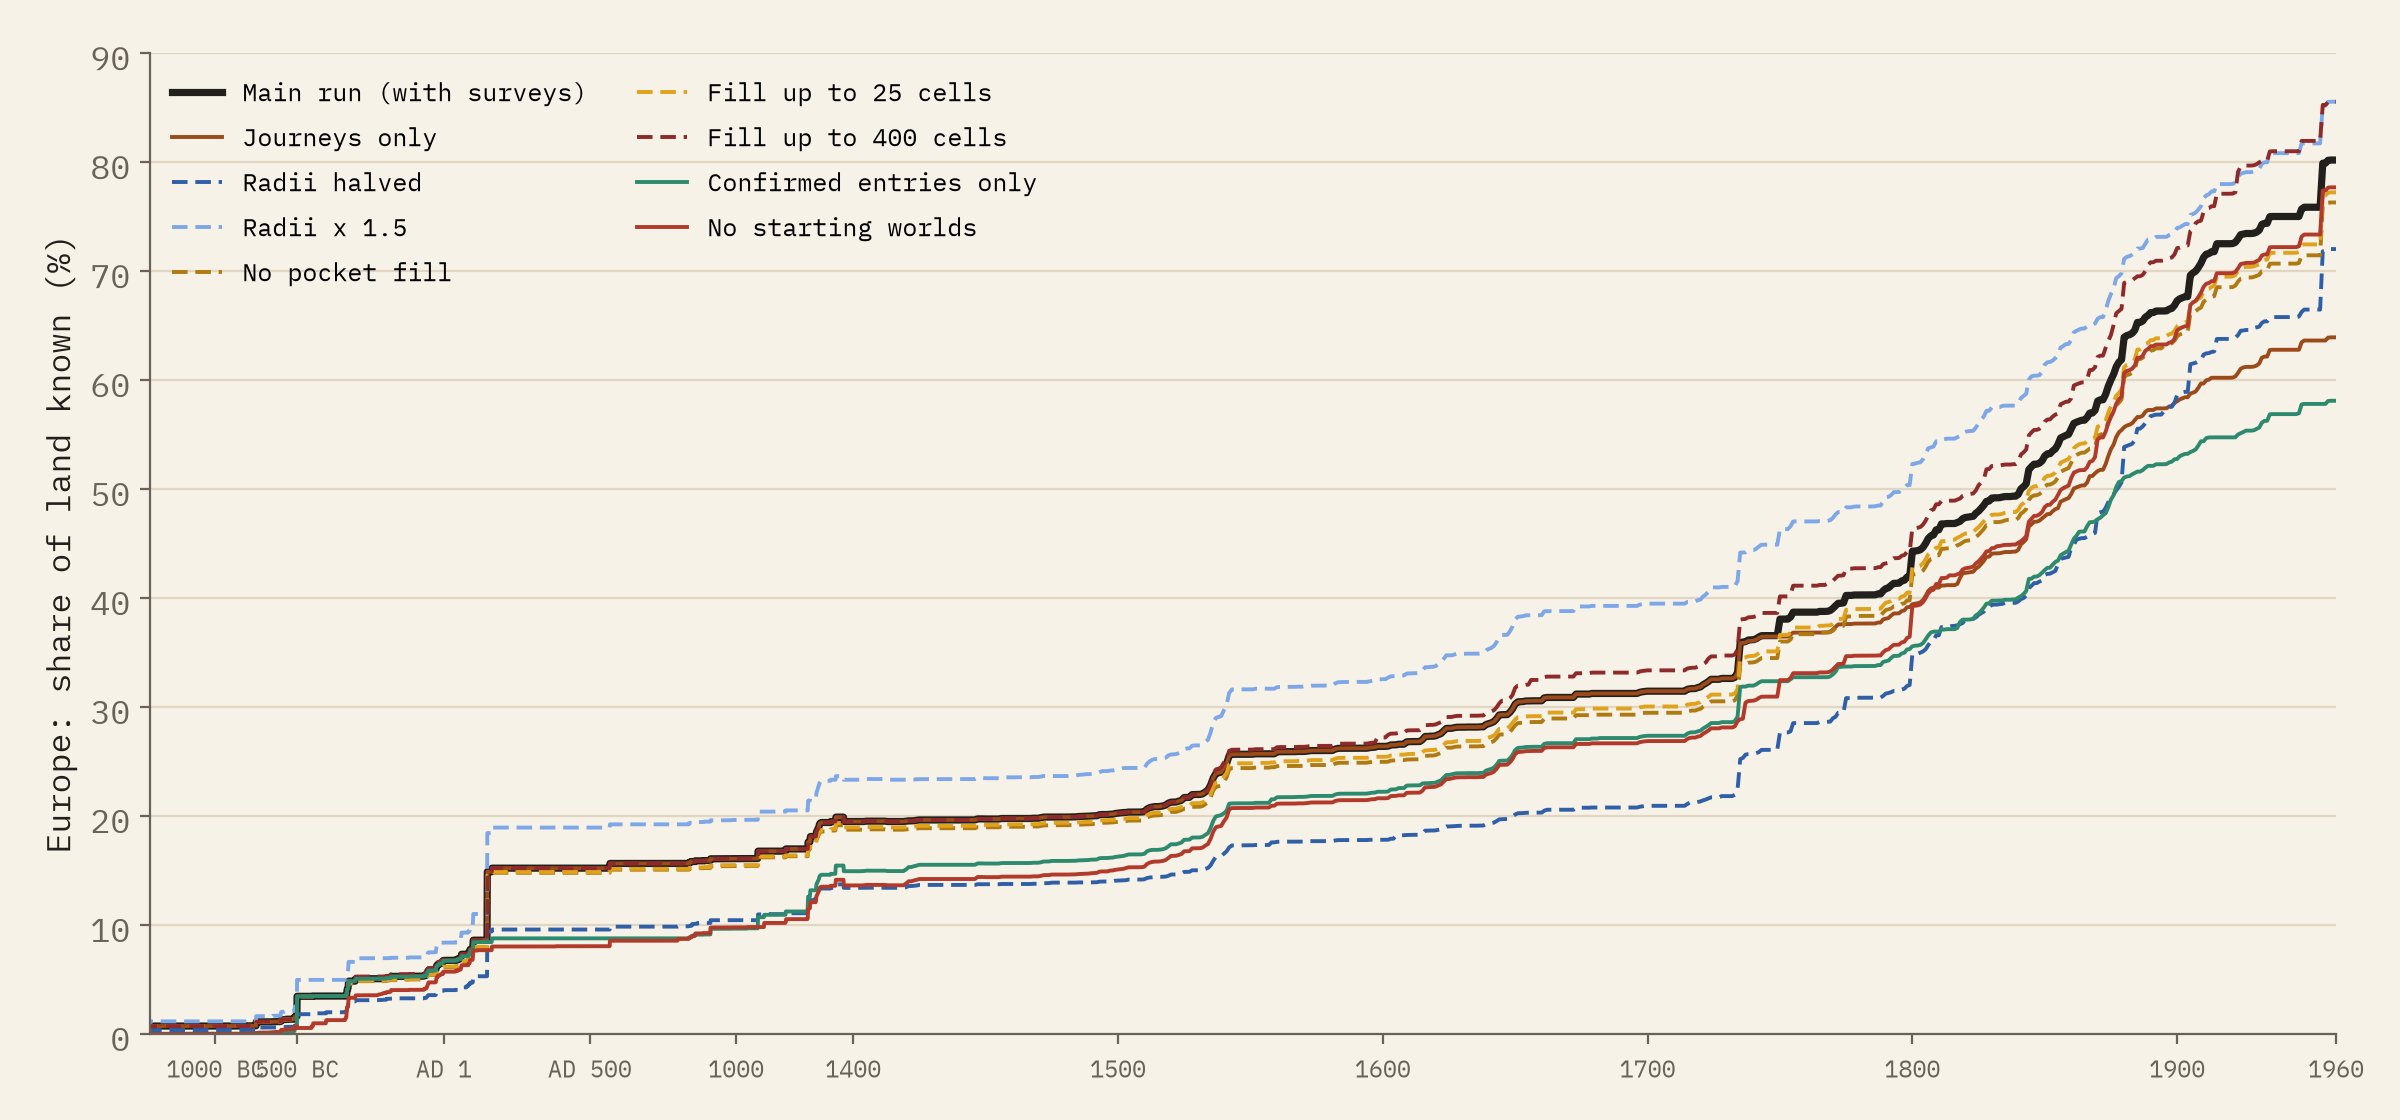
\includegraphics[width=\textwidth]{f_sensitivity.png}
\caption{Europe's share of land known under each variant of the model.}\label{fig:sens}\end{figure}

\begin{figure}[tbp]\centering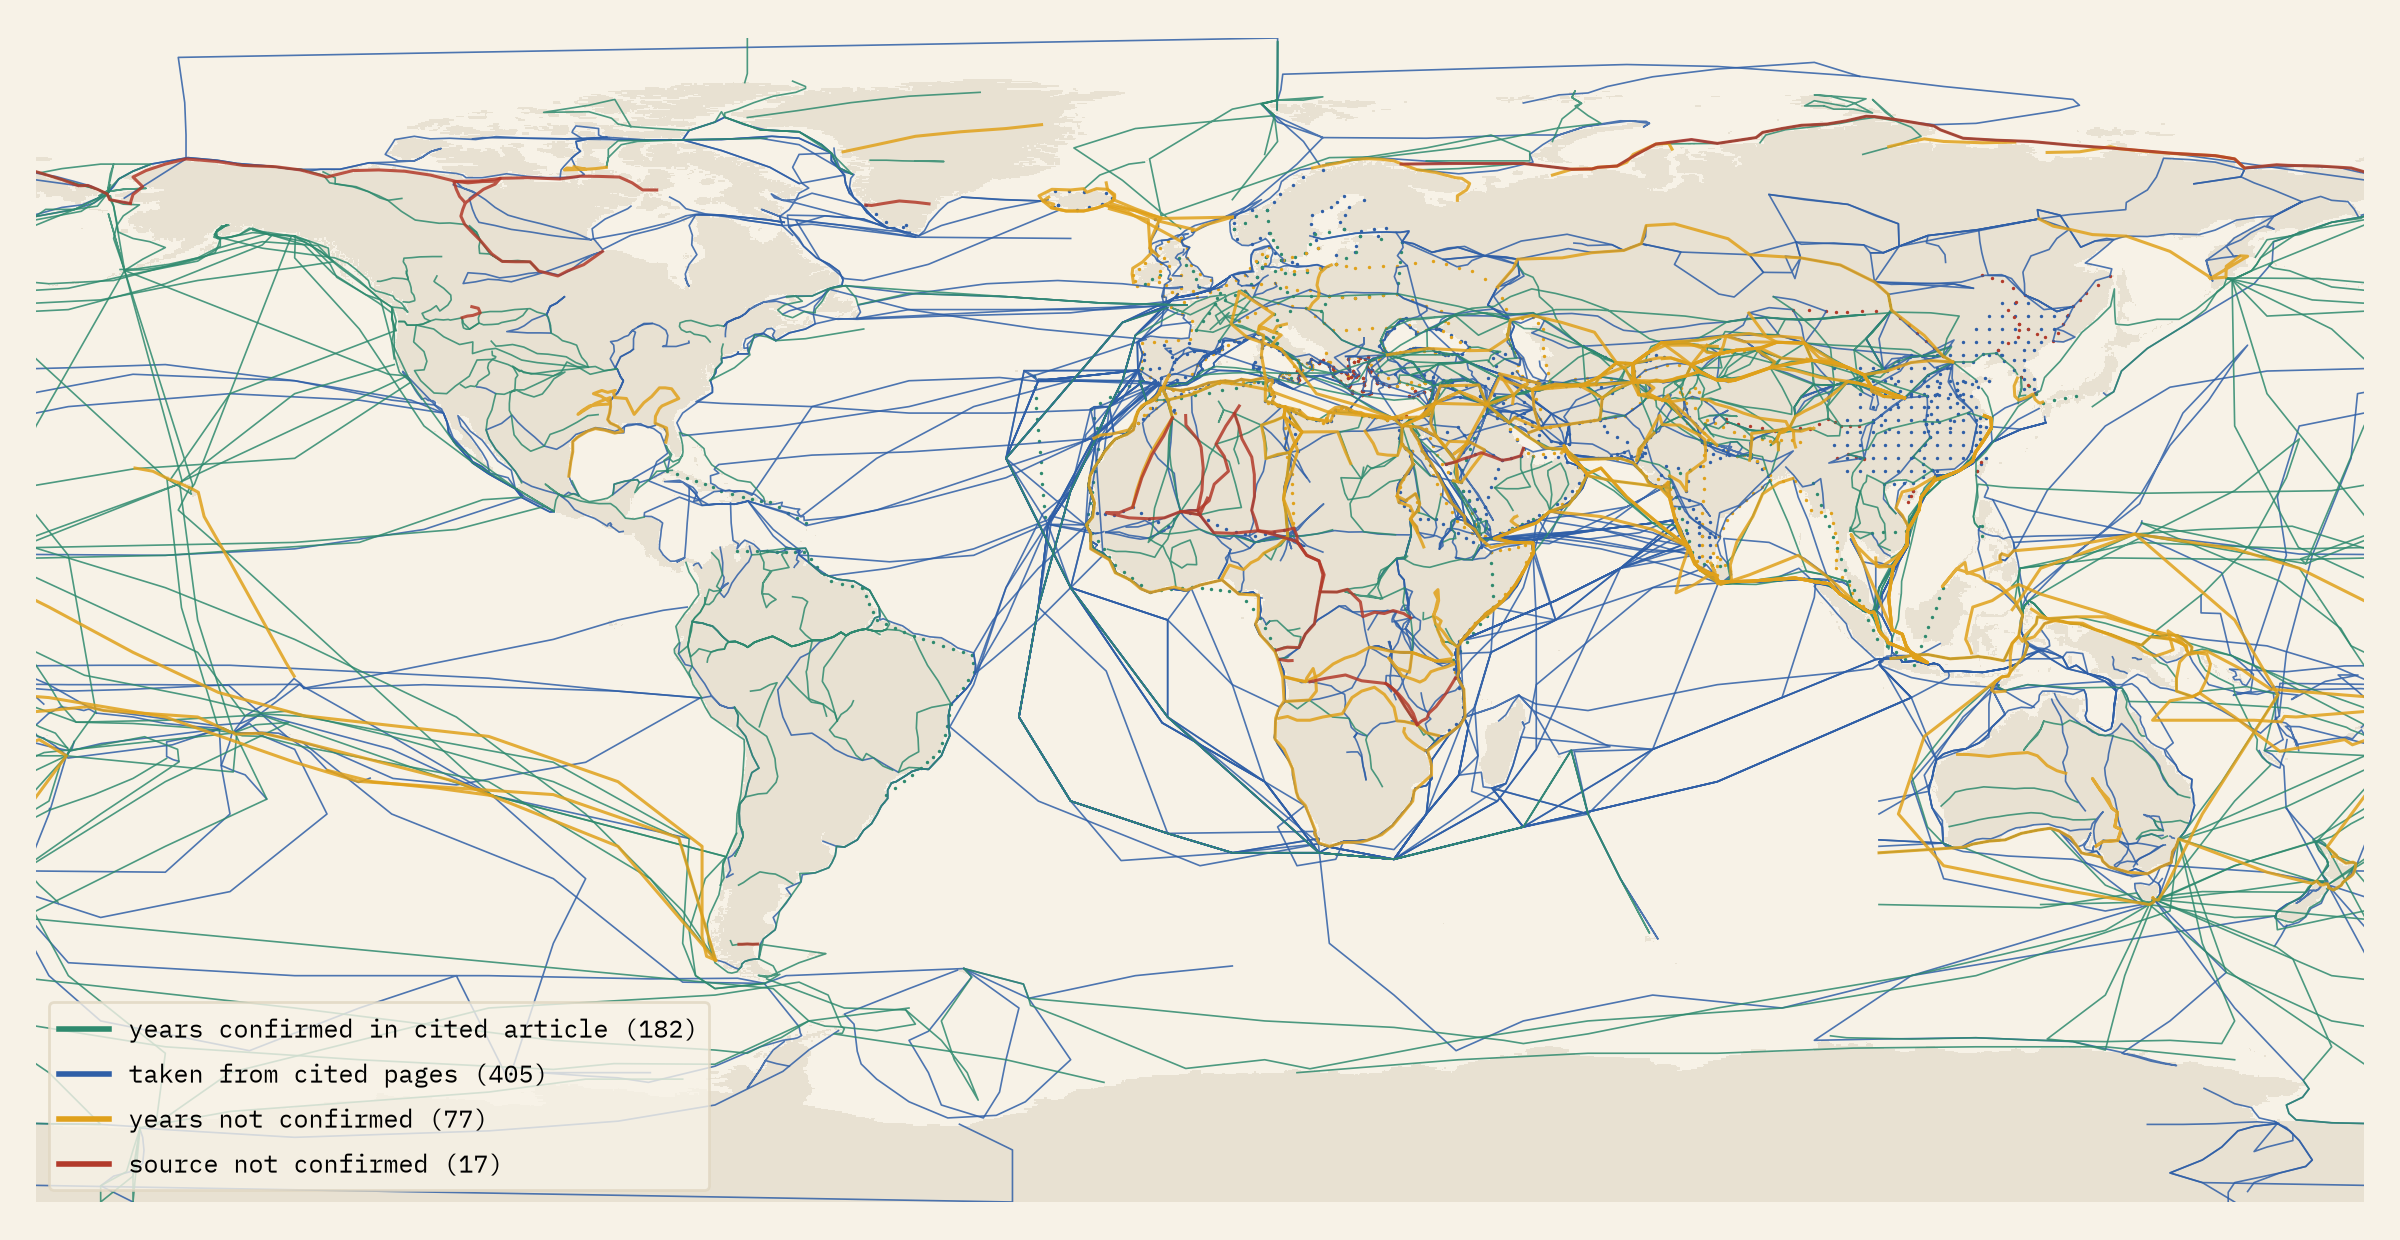
\includegraphics[width=\textwidth]{f_status.png}
\caption{All routes coloured by source status. Dots: starting-world entries.}\label{fig:status}\end{figure}

\section{Limitations}
The measure is the area near journeys in one gazetteer, not what any society knew. The gazetteer was compiled with AI assistance from mostly English-language sources, especially Wikipedia, which document European explorers far better than Arabic, Persian, Chinese or Pacific traditions; the other viewpoints are therefore thinner than they should be, and comparisons between traditions are indicative only. Journeys are dated by when they happened, not when their accounts were published or read, and the reach of an account (who read it, and whether it was believed) is not modelled. The survey and settlement layer is coarse, its dates unconfirmed, and it exists only for Europe; trade networks and missions are absent, so late shares remain lower bounds and comparisons with other traditions after 1700 favour Europe by construction. Routes are simplified and some are reconstructed. A fixed reveal distance treats a desert crossing, a forest river and a coast seen through fog alike. Starting worlds are coarse, and the base radius can light coasts more widely than the voyages that preceded them. Around 11\% of entries have unconfirmed years and 2.5\% unconfirmed sources; they are flagged, and removing them does not change the conclusions.

\section{Conclusion}
Measured this way, Europe's recorded world grew in three phases: a classical expansion that ended with Ptolemy, about a millennium of near standstill, and five centuries of growth that lit the oceans first and the continental interiors last, fastest in the nineteenth century. The same method applied to other traditions shows how much of the ``unknown'' of the European map was recorded elsewhere first, from the Chinese interior to the Polynesian Pacific. The numbers depend on modelling choices and on the coverage of the gazetteer, both of which are published so that they can be challenged and improved.

\section*{Data and code availability}
The interactive version is at \url{https://maps.tristanhotham.com/known-world/}. Data and code are at \url{https://github.com/Tristan-Hotham/known-world} and archived with this paper at https://doi.org/10.5281/zenodo.23897793. Derived data are released under CC BY 4.0 and code under the MIT licence; the journey gazetteer, which draws on Wikipedia, is released under CC BY-SA 4.0.

\section*{AI statement}
I wrote the text, with drafting and editing assistance from Claude (Anthropic), which also helped prepare the analysis code. I reviewed and checked all text and results.

\begin{thebibliography}{9}
\bibitem[Natural Earth(2026)]{naturalearth} Natural Earth (2026) Land, Antarctic ice shelves, Admin 0 countries and populated places, 1:50m and 1:10m. Public domain. \url{https://www.naturalearthdata.com/}
\bibitem[Uber(2026)]{h3} Uber Technologies (2026) H3: a hexagonal hierarchical geospatial indexing system. Apache 2.0. \url{https://h3geo.org/}
\bibitem[Wikipedia(2026)]{wiki} Wikipedia contributors (2026) Articles on individual journeys and travellers, as cited per journey in the gazetteer. CC BY-SA 4.0. \url{https://en.wikipedia.org/}
\end{thebibliography}
\end{document}
